\documentclass[a4paper,12pt]{article}
\usepackage{palatino}
\usepackage{graphicx}
\usepackage{amsmath}
\usepackage[margin=1.5cm,
    vmargin={0pt,1cm},
    includefoot]{geometry}

\title{Demonstration Document}
\author{M. Y. Self\\
        At Home}
\date{February 1, 2004}

\begin{document}

\maketitle

\section{Introduction}

\subsection{Simple text}
This first section contains simple text.
On input, lines can be broken wherever one pleases,
  with extra spacing included to improve legibility,
  but the output lines will be broken to fit the
  line width available. Even additional    spacing
     between    words   does   not    affect
        the output.

A new paragraph in indicated with a blank line.

\subsection{Highlighting text}

It is possible to emphasize text by setting it in
\emph{italic} or in \textbf{boldface}.

\begin{quote}
Another possibility is to offset a piece of text in a
\texttt{quote} environment like this, with increased
margins on either side.
\end{quote}

\section{Sophistications}

\subsection{Mathematics}

There are special rules for entering math, and many
commands that only exist in math mode. An in-line math
formula like $x^2+\beta$ has automatic spacing between
variables and operators, while displayed equations like
\begin{equation}
  \vec{A} \times (\vec{B}\times\vec{C}) =
  (\vec{A}\cdot\vec{C})\vec{B} -
  (\vec{A}\cdot\vec{B})\vec{C}
\end{equation}
\begin{equation}
  \vec{A}\cdot(\vec{B}\times\vec{C}) =
  \begin{vmatrix}
    A_x & A_y & A_y \\
    B_x & B_y & B_y \\
    C_x & C_y & C_y
  \end{vmatrix}
\end{equation}
are given automatic numbers.

\subsection{Lists}

\begin{enumerate}
\item Various lists are possible, to enumerate,
\item to itemize with bullets,
\item or to make descriptive lists.
\end{enumerate}

\subsection{Adding graphics}

Pictures and graphics
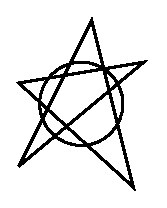
\includegraphics[width=1cm]{demo}
produced by other programs are easily inserted.
\end{document}
